\section{Problem 2: PCB Layout}
The goal of this exercise is to place 14 different chips on two PCB
boards, without the chips overlapping with another chip, battery, or
camera. However, certain chips are prone to overheating and cannot be
placed near each other. Keeping these constraints in mind, is it
possible to find a valid placement of the chips for 3 different PCB
designs?

    \subsection{Solution}
            
        \subsubsection{Constants}
            \begin{itemize}
                \item $n=14$, the number of chips that need to be placed
                \item $m = 3$, the number of objects on the PCB
            \end{itemize}

            \begin{table}[h]
                \centering
                \begin{tabular}{l|cccccccccccccc}
                \toprule
                \multicolumn{15}{c}{Chips} \\
                \midrule
                width & 5 & 5 & 4 & 4  & 5 & 3 & 7 & 6  & 6  & 4  & 6 & 5  & 6  & 5  \\
                height& 6 & 6 & 6 & 10 & 7 & 7 & 7 & 10 & 12 & 10 & 9 & 11 & 10 & 10 \\
                hot?  & \checkmark & \checkmark & & & & \checkmark & & & & & & & &   \\
                \bottomrule
                \end{tabular}
            \end{table}

            It is possible for the PCB's to contain objects like batteries or 
            camera's, just like the different chip sizes these objects are part of
            the PCB design that are already determined by the problem description.

            \begin{table}[h]
                \centering
                \begin{tabular}{l|cccccc}
                \toprule
                \multicolumn{6}{c}{Objects} \\
                \midrule
                label      & Battery & Battery & Camera A & Camera B  & Camera C \\
                width      & 12 & 14 & 7 & 11  & 15 \\
                height     & 8 & 12 & 5 & 5 & 5 \\
                x position & 0 & 0 & 17 & 13 & 9 \\
                y position & 0 & 0 & 22 & 22 & 22 \\
                PCB        & 1 & 2 & 2 & 2  & 2 \\
                \bottomrule
                \end{tabular}
            \end{table}

    \subsection{Variables}

        We use different parameters for the problem:
        
        \begin{itemize}
            \item $n=$ the number of chips that need to be placed
            \item $m = $ the number of objects on the PCB
        \end{itemize}

        For $i \in \{0, 1, ..., n-1\}$, we have the following variables:
        \begin{itemize}
            \item $X_i$ representing the $x$ coordinate of the lower left corner
                of chip $i$.
            \item $Y_i$ representing the $y$ coordinate of the lower left corner
                of chip $i$.
            \item $R_i$ representing whether a a chip $i$ is rotated.
            \item $W_i$ representing the width of the chip $i$.
            \item $H_i$ representing the height of chip $i$.
            \item $PCB_i$ representing the PCB where chip $i$ is placed on.
            \item $Hot_i$ representing whether chip $i$ becomes warm under load.
        \end{itemize}

        We further expand on these variables by defining values for the $x$ and
        $y$ intervals, these will aid us in detecting overlaps:
        
        $$X_i^{min} = X_i$$

        $$
        X^{\max}_{i} = \begin{cases} 
            X_i + W_i & \text{if } R_i = 0, \\
            X_i + H_i & \text{otherwise}
        \end{cases}
        $$

        Repeat the same procedure for $Y^{min}_i$ and $Y^{max}_{i}$

        Lastly we use these properties not only for the chips but also for the
        objects that can be placed upon the PCB like the battery or camera's.
        For a range $i \in \{0, ..., m-1\}$, we define the variables as
        follows, $X_i^o$, $Y_i^o$, $R_i^o$, $W_i^o$, $H_i^o$, but defined with
        the superscript $o$, to differentiate between the chip related
        variables.

        To build up the CNF which will solve the PCB layout problem we use the
        variables mentioned above, to construct the following placement
        constraints:

        \begin{itemize}
            \item Chips cannot overlap
            \item Chips should be placed on the PCB
            \item Chips cannot overlap with Objects
            \item Chips that produce heat cannot be placed near each other.
        \end{itemize}

    \subsection{Constraints}
        
        \subsubsection{Chip Overlap}

            \begin{itemize}
                \item Overlap constraint:
                    \[
                        \bigwedge_{i=0}^{n}\bigwedge_{j=0}^{n} \lnot Overlap(i, j)
                    \]

                    $Chip_i$ and $Chip_j$ overlap only if they overlap in the
                    x-intervals, y-intervals and are placed on the same PCB.
                    
                    \[  
                        Overlap(i,j) = 
                        Overlap_x(i, j) \land
                        Overlap_y(i, j) \land
                        PCB[i] = PCB[j]
                    \]

                    We check for overlap on the x-interval with the following
                    equation:

                    \[
                        Overlap(i, j) : 
                        x_i^{min} < x_j^{max} \land x_i^{min} < x_j^{max}
                    \]
                    
                    Repeat the process for the y direction.

            \end{itemize}

            $$
            \begin{aligned}
                & (R[j] = 0 \land X[i] < X[j] + W[j]) \lor (R[j] \neq 0 \land
                X[i] < X[j] + H[j]) \\
                \land \;& (R[i] = 0 \land 
                X[j] < X[i] + W[i]) \lor (R[i] \neq 0 \land X[j] < X[i] + H[i])
            \end{aligned}
            $$

            With $\mathrm{Overlap}$ for a particular axis being defined as:

            $$
            \mathrm{Overlap}_x(i,j) = X^{\mathrm{min}}_i < X^{\mathrm{max}}_j
            \land X^{\mathrm{min}}_j < X^{\mathrm{max}}_i 
            $$

        \subsubsection{Placed on PCB}

            \begin{itemize}
                \item The chips placed should be placed within the bounds of the
                PCB:

                \[
                    PlacedOnPCB(i) = \begin{cases}
                        X_i^{max} \leq W^{PCB_1}_i \land 
                        Y_i^{max} \leq H^{PCB_1}_i & \text{if } PCB_i = 1, \\
                        X_i^{max} \leq W^{PCB_2}_i \land
                        Y_i^{max} \leq H^{PCB_2}_i & \text{otherwise}
                    \end{cases}
                \]
            \end{itemize}

        \subsubsection{No overlap with PCB Objects}

            \[
                \bigwedge_{i=0}^{n}\bigwedge_{j=0}^{m} \lnot PCBOverlap(i, j)
            \]

            Here, $PCBOverlap$ is defined similarly as $Overlap$ between chips,
            differing only in how the $j$ variable is used as an index for the
            $X_j^o$, $Y_j^o$, $R_j^o$, $W_j^o$, $H_j^o$ variables. For brevity,
            this is omitted from the report.

        \subsubsection{Is Overheating}

            \begin{itemize}
                \item 
                Chips that overheat must have their centers placed at least 20
                units away from both the x and y axes.
                
                $$
                \bigwedge_{i=0}^{n}\bigwedge_{j=0}^{n} \lnot IsOverheating(i,j)
                $$

                Let $x_i^{center}$ be the the center of the interval
                $(X_i^{min}, X_i^{max})$, repeating the same process for the
                variables for the $y$-axis 

                \[
                IsOverheating(i,j) = |X_i^{center}-X_i^{center}| \leq 20 \land
                |Y_i^{center}-Y_i^{center}| \leq 20 \land PCB_i = PCB_j \land
                Hot_i \land Hot_j
                \]
            \end{itemize}

    \subsection{Results:}

        \subsubsection{Visualization Exercise 2a}

            \begin{figure}[H]
                \centering
                \begin{minipage}{0.45\textwidth}
                    \centering
                    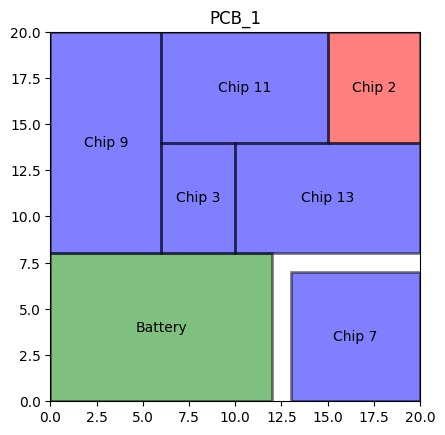
\includegraphics[width=\linewidth]{assets/pcb-1-a.jpeg}
                    \caption{PCB 1, with Camera A}
                    \label{fig:pcb1}
                \end{minipage}\hfill
                \begin{minipage}{0.45\textwidth}
                    \centering
                    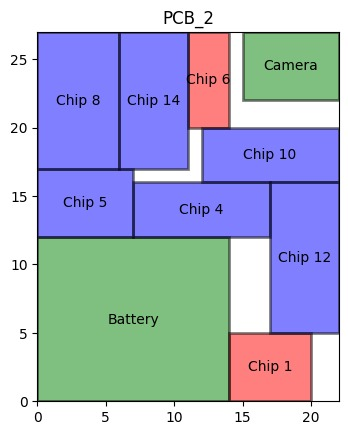
\includegraphics[width=\linewidth]{assets/pcb-2-a.jpeg}
                    \caption{PCB 2, with Camera A}
                    \label{fig:pcb2}
                \end{minipage}
            \end{figure}

            \subsubsection{Visualization Exercise 2b}
            \begin{figure}[H]
                \centering
                \begin{minipage}{0.45\textwidth}
                    \centering
                    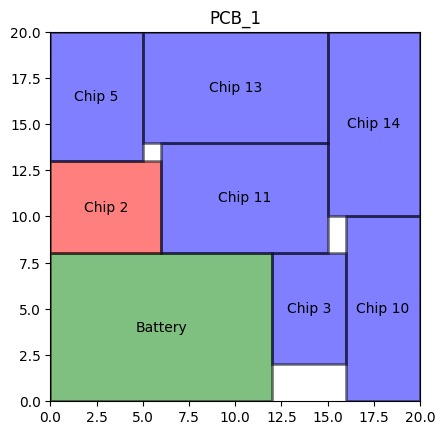
\includegraphics[width=\linewidth]{assets/pcb-1-b.jpeg}
                    \caption{PCB 1, with Camera B}
                    \label{fig:pcb1b}
                \end{minipage}\hfill
                \begin{minipage}{0.45\textwidth}
                    \centering
                    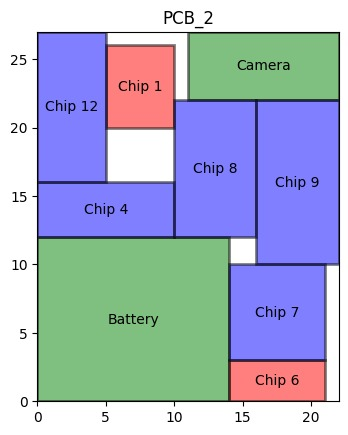
\includegraphics[width=\linewidth]{assets/pcb-2-b.jpeg}
                    \caption{PCB 2, with Camera B}
                    \label{fig:pcb2b}
                \end{minipage}
            \end{figure}

            \subsubsection{Visualization Exercise 2c}

            \begin{itemize}
                \item UNSAT
            \end{itemize}
